\subsection{Applications}
\label{architecture_s}	


The overall objective is to allow a client to trust a code produced by an untrusted code producer. Our approach is especially suitable
 in cases where the client policy involves non trivial functional or safety requirements and thus, a full automatization of the verification 
process is impossible. To this end, we propose a PCC technique that exploits the JML compiler and the weakest predicate function presented in the article. 
 
 The framework is presented in Fig.~\ref{architecture}; note that certificates and their checking are not yet implemented
 and thus are in oblique font.
  


 \begin{figure}[!tbp]
 \centering
\epsfig{ file=sac/architecture.eps, width=3in, height=3in }
%\includegraphics[width=3in,height=3in]{architecture}  
\caption{\sc The overall architecture for client producer scenarios }
\label{architecture}
\end{figure}




%\clearpage

In the first stage of the process the client provides the functional and (or) security requirements to the producer.
 The requirements can be in different form:
\begin{itemize}
\item Typical functional requirements can be a specified interface describing the application to be developed. 
In that case, the client specifies in JML the features that have to be implemented by the code producer.
\item Client security requirements can be a restricted access to some method from the API expressed as a finite state machine.
For example, suppose that the client API provides transaction management facilities - the API method \texttt{open} for opening and method 
\texttt{close} for closing transactions. In this case, a requirement can be for no nested transactions.
This means that the methods \texttt{open} and \texttt{close} can be annotated to ensure that the method \texttt{close} 
 should not be called if there is no transaction running and the method \texttt{open} should not be called if there is already a running transaction. 
In this scenario, we can apply results of previous work \cite{m+04:cardis}.  
\end{itemize}

Usually, the development process involves annotating the source code with JML specification,
 generating verification conditions, using proof obligation generator over the source code and 
discharging proofs which represent the program safety certificate and finally, the producer sends the certificate 
to the client along with the annotated class files.
 Yielding certificates over the source code is based on the observation that
 proof obligations on the source code and non-optimized bytecode respectively
 are syntactically the same modulo names and basic types. Every Java file of the 
untrusted code is normally compiled with a Java compiler to obtain a class file. Every class file is extended with
 user defined attributes that contain the BCSL specification, resulting from the compilation of the
 JML specification of the corresponding Java source file.



    

% If the annotations are sufficient to prove the code, 
%the Java file is normally compiled with a Java compiler to obtain a 
%class file. This class file is then extended with user defined attributes that contain the BCSL specification, 
%resulting from the compilation of the JML specification in the Java source file. 
%At this stage, the Java class files contain all the information that will allow the client to check if the bytecode does not violate 
%his requirements. 


%Actually, our early experiments show that the proof obligations on source and bytecode level are syntactically modulo names and types.   

%OLD
%To implement this architecture, we have defined a compiler from JML to BCSL; the JML compilation results in an extension of the class file format; 
%we have implemented a tool to insert those special attributes in the class file and we have extended the JACK framework to generate proof obligations at bytecode 
%level and to prove them with the plugged JACK provers (as explained in the introduction). 
%The coming sections introduce those features.  

To implement this architecture we use JACK~\cite{BRL-JACK} as a verification condition generator both on the consumer and the
producer side. JACK is a plugin for the eclipse\footnote{http://www.eclipse.org} integrated development environment for Java.
 Originally, the tool was designed as verification condition generator for Java source programs against their JML specification.
 JACK can interface with several theorem provers (AtelierB, Simplify, Coq, PVS). We have extended the tool with a compiler from
 JML to BCSL and a bytecode verification condition generator. In the next sections, we introduce
 the BCSL language, the JML compiler and the bytecode \wpi calculus which underlines the bytecode verification condition generator.
 
%the JML compilation results in an extension of the class file format; we have implemented a tool to insert those special attributes in the class file and we have extended 
%the JACK framework to generate proof obligations at bytecode level and to prove them with the plugged JACK provers (as explained in the introduction). 
%The coming sections introduce those features.  
